\documentclass{sem5}
\usepackage{caption}
\institutename{Indian Institute of Information Technology, Vadodara}
\author{Dilip Puri}
\idt{201351014}
%\team{teamname}
\collab{\textbf{Collaborators} - Hemant Kumar(201352026)\\ Govind Meena(201352010)}

\coursename{Parallel Programming}
\ccode{\begin{small}CS403\end{small}}
\profname{Prof. Reshmi Mitra}

\type{Project}
\typeid{1}
\submissiondate{\today}%dd/mm/yyyy
\deadline{Sep12, 11.59 PM}%dd/mm/yyyy @hh:mm pm/am
\problemset{LU Decomposition}

\begin{document}

\section{Introduction}
Let A be a square matrix. If there is a lower triangular matrix L with all diagonal entries equal to 1 and an upper matrix U such that A=LU, then we say that A has an LU-decomposition. It can be helpful in calculating various types of operation on matrices. Here L matrix has the upper triangular values as 0 and U has lower triangular values as 0 and diagonal values same as that of the original matrix. 

\section{Algorithm}
\begin{figure}[htbp]
\centering
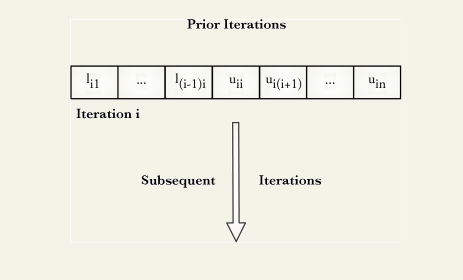
\includegraphics[scale=.5]{1.png}
\caption{Computational Sequence of Doolittle's Method}
\end{figure}
\begin{figure}
\centering
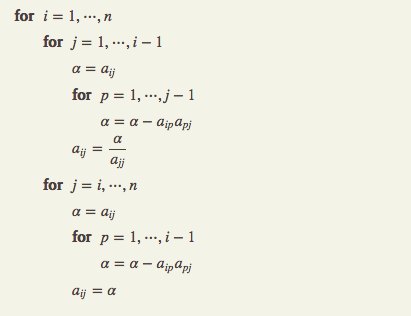
\includegraphics[scale=.5]{2.png}
\caption{Doolittle's LU Decompostion Algorithm}
\end{figure}
\newpage
\section{Serial Code}
\lstinputlisting[frame=single, basicstyle=\small\ttfamily, caption=Code, language=C]{../lu.c}
\section{Analysis using Valgrind}

\end{document}